\lstdefinestyle{yaml}{
     basicstyle=\color{blue}\footnotesize,
     rulecolor=\color{black},
     string=[s]{'}{'},
     stringstyle=\color{blue},
     comment=[l]{:},
     commentstyle=\color{black},
     morecomment=[l]{-}
 }
\chapter{Communication architecture}

In this chapter, we will elaborate on how the components mentioned in earlier chapters interact with each other. Additionally, we will indicate the steps we've followed to deploy the web application on a cloud environment.
Using the MQTT protocol, the rover and the web application do not need direct connection to interact with each other. Instead, the MQTT broker acts as a middleman that sends the most recent information on each topic to its respective subscribers. Whenever a user connects to the web application, the back-end provides the views defined in the front-end as the visible interface and handles the interactions with the database where our photos are stored and accessed. These interactions are shown in the following chart:
\begin{figure}[H]
    \centering
    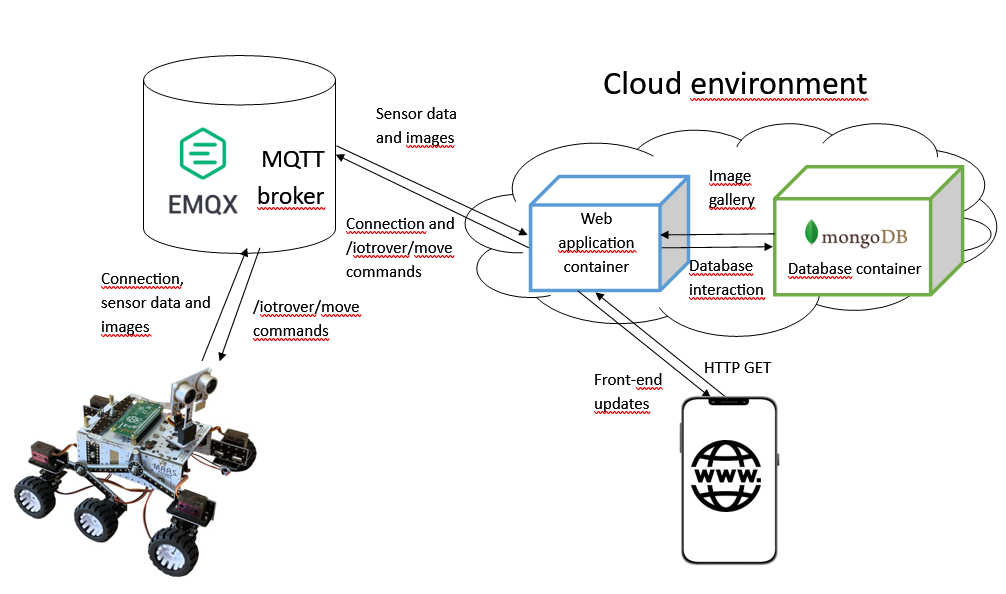
\includegraphics[width=1\linewidth]{connectionchart.png}
    \caption{Chart showcasing the different connections between components}
    \label{fig:enter-label}
\end{figure}
\section{Cloud Deployment}

As the final step in the development of our project, we have decided to deploy our web application, along with a database, on a cloud service. For this purpose, we requested access to an environment on the THM's cloud platform. With this environment, we can deploy our application on a virtual container, allowing access to it anywhere on the THM's local network. In this environment, which was managed through a web interface called Portainer, we were granted the following permissions:
% Docker should be explained better on the first Kapitel
\begin{itemize}
    \item Pull virtual container images from a public repository hosted on Docker Hub, the official repository for images.
    \item Create and manage our own containers, provided we set them up on the ports we were granted during the lab sessions done prior to the project.
    \item Create volumes for storing data, without the ability to directly manage them.
    \item  Create and manage a group to grant access to all the group members to the deployed stacks or containers.
\end{itemize}

These limitations had to be taken into account when designing the deployed systems. In the end, we opted for two virtual containers; one hosting the web application and the other for hosting the MongoDB database. Furthermore, we deployed both containers at once using a stack, which allows for an easier and more personalized deployment as one application that has two services. The following sections will discuss the idiosyncrasies of every part of this deployment.

\subsection{Web application container}

In order to deploy the web application on a virtual container, we needed both an image for the container and a way to make the assets of our project available to it. Unfortunately, because we could not manage a volume and constantly update it, we instead opted with copying the files when building the image, which required building it and updating it every time we made changes on the application.

The steps needed to build the image and the resulting container's behavior can be defined with a file named Dockerfile. This is the one we used for our image, and we placed on the application's root folder:

\begin{lstlisting}
# Use official Node.js LTS image
FROM node:18-alpine

# Set working directory
WORKDIR /app

# Copy package.json and package-lock.json
COPY package*.json ./

# Install dependencies
RUN npm install

# Copy the rest of the application
COPY . ./
# Expose the application port (change if needed)
EXPOSE 3000

# Command to run the application
CMD ["node", "app.js"]
\end{lstlisting}

We then run on the same folder on a terminal the command docker build . -t relr82/iot-project2024-backend. This command creates an image based on the Dockerfile and assigns it the name relr82/iot-project2024-backend. If everything goes well, we should see this on our local Docker Desktop:
\begin{figure}[H]
    \centering
    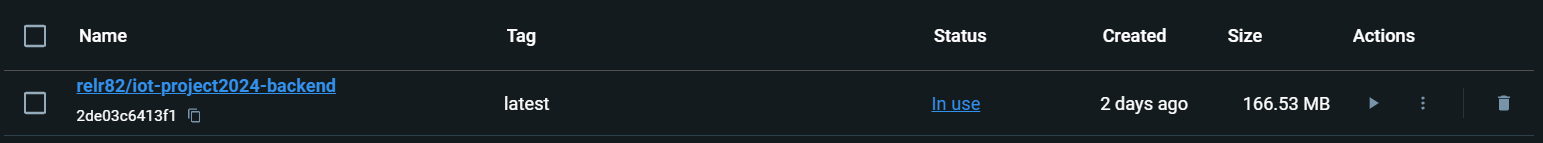
\includegraphics[width=1\linewidth]{dockerdesktop.png}
    \caption{Image of the resulting image on Docker Desktop}
    \label{fig:enter-label}
\end{figure}

To make it easier to update the image, we created a public online repository in Docker Hub. We can push updates to this repository by authenticating running docker login and then running docker push relr82/iot-project2024-backend. This pushes the image to the repository.

\begin{figure}[H]
    \centering
    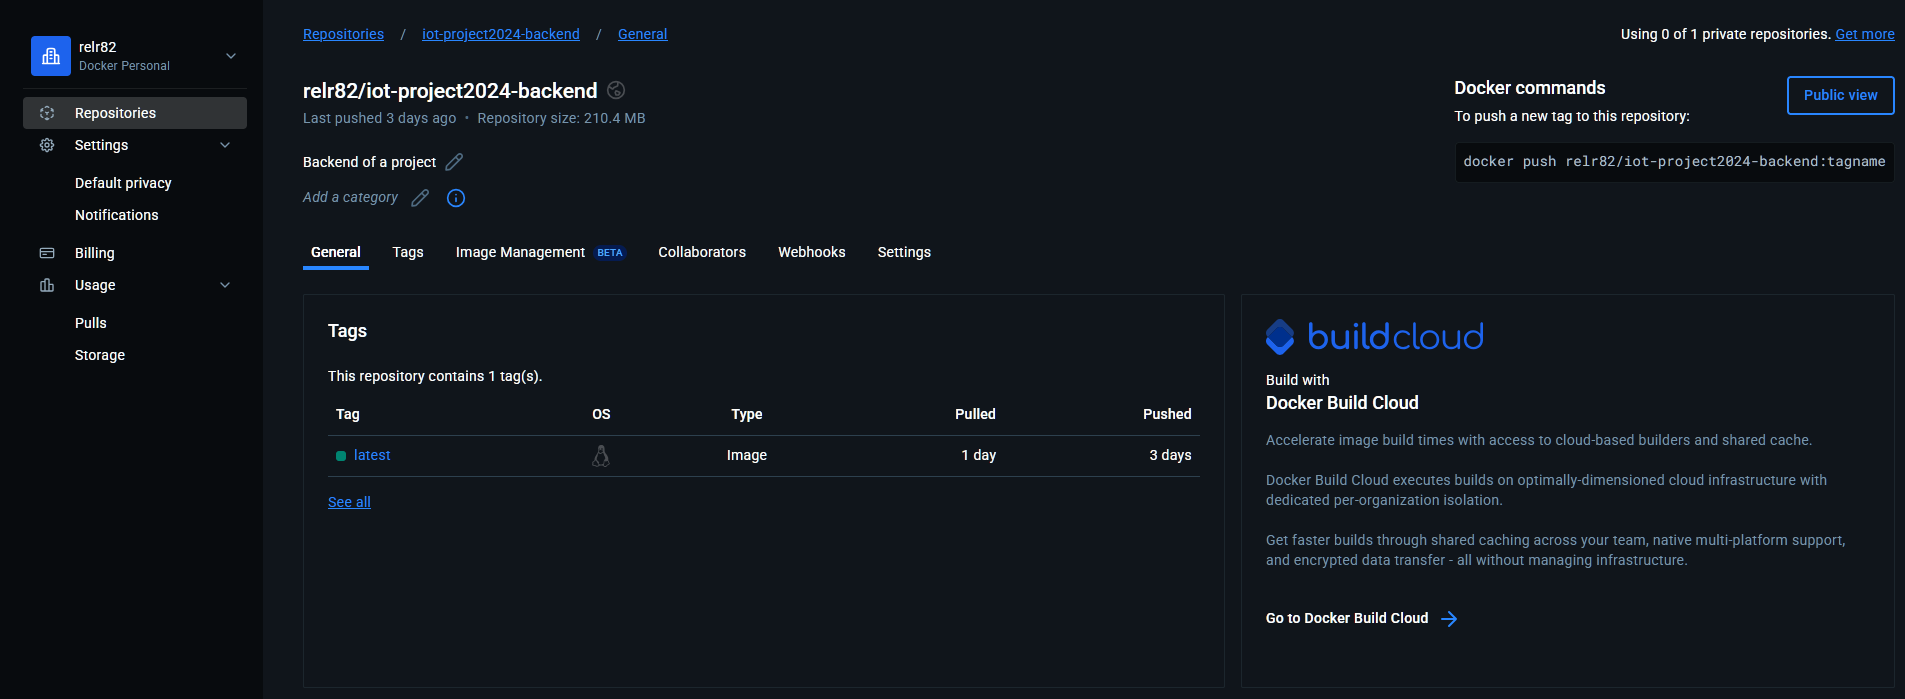
\includegraphics[width=0.5\linewidth]{dockerhub.png}
    \caption{Docker Hub repository where we push our image}
    \label{fig:enter-label}
\end{figure}

Whenever we want to access it in our stack, we just need to call that image followed by the tag :latest to use the latest version available and indicate to re-pull all images when updating the stack in Portainer.

\subsection{MongoDB container}

To complement the web application, we deploy a MongoDB database in a virtual container. This database can be easily deployed using the public MongoDB Docker image. However, we have to be extremely wary of how MongoDB allocates resources. For starters, MongoDB uses ALL the available RAM regardless of how we limit it through resource limits. So along with it, we have to ensure MongoDB executes with the flag --wiredTigerCacheSizeGB 0.25. This limits the amount of cache available by wiredTiger, MongoDB's default storage engine. For good measure, we also limit the memory usable by the container on the stack. 

\subsection{Stack}

Finally, we set up the stack in Portainer. Stacks in docker are defined using a docker-compose file written in YAML notation. On this file, we define each container as a service with different properties, along with the volumes and networks used by them. On the web application service (called backend), we indicate the image mentioned earlier. We also define the database used as an environment variable called URL and map the used well-known port to one of ours outside the stack (not doing so will block Portainer from working).
For the mongoDB database, we apply the resource limitations we mentioned earlier and define a volume for the database information. Below is the docker-compose file that builds the stack:

\begin{lstlisting}[style=yaml]
version: "3.1"

services:
  backend:
    image: relr82/iot-project2024-backend:latest
    restart: always #Always restarts backend service
    stdin_open: true # docker run -i
    tty: true        # docker run -t
    environment:
      - URL=mongodb://mongo:27017/dbname
    ports:
      - "50234:3000" #Maps exposed port to a not well-known port
    deploy:
      resources:
        limits:
          cpus: '0.5'
          memory: 50M
  mongo:
    image: mongo:latest
    container_name: gr3_mongo
    stdin_open: true # docker run -i
    tty: true        # docker run -t
    command: --wiredTigerCacheSizeGB 0.25
    ports:
      - "50233:27017"
    volumes:
      - gr3_mongo_vol:/data/db
    deploy:
      resources:
        limits:
          cpus: '0.5'
          memory: 256m 
    mem_limit: 256m 


volumes:
  gr3_mongo_vol:  
 

networks:
  gr3_net: 

\end{lstlisting}

After creating the stack, we should see two containers being deployed:
\begin{figure}[H]
    \centering
    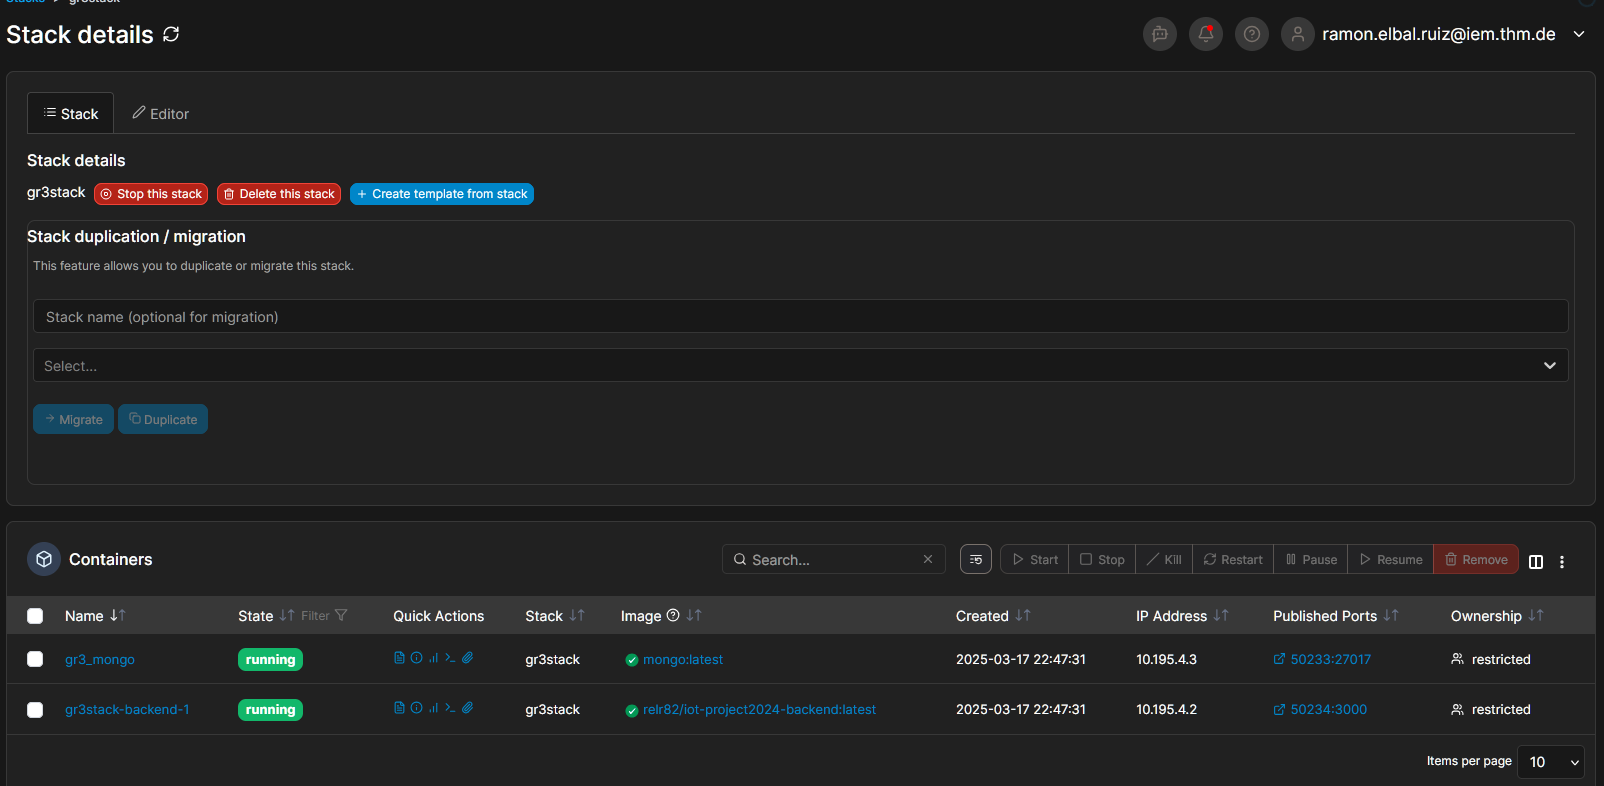
\includegraphics[width=0.5\linewidth]{stack.png}
    \caption{Stack being deployed on Portainer}
    \label{fig:enter-label}
\end{figure}

To access the web application, we have to use the URL of our environment and the port we mapped the service to. The following image shows an example in which the web application is not only operational on the cloud but able to communicate with the MongoDB database deployed in our container.
\begin{figure}[H]
    \centering
    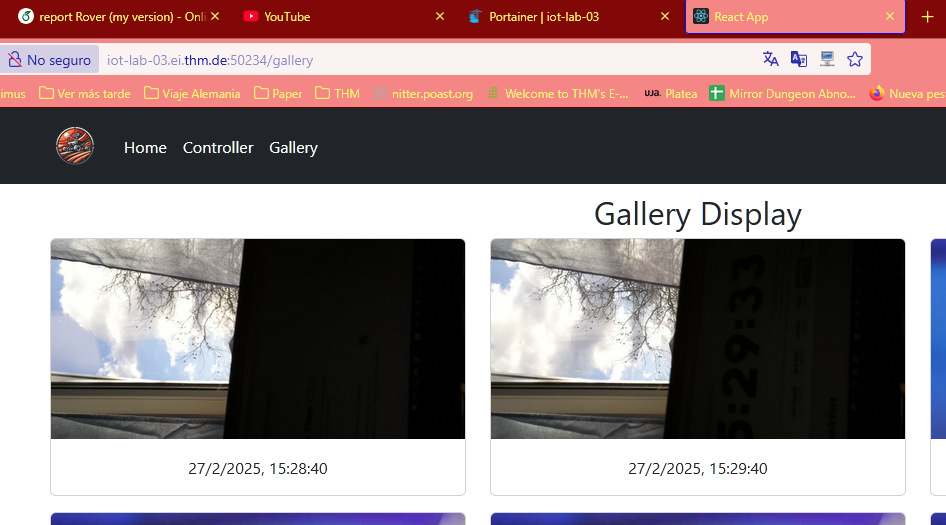
\includegraphics[width=0.5\linewidth]{clouddemo.png}
    \caption{Demonstration of the web application running and accessing the database}
    \label{fig:enter-label}
\end{figure}